\documentclass[10pt]{beamer} 
\usetheme{PaloAlto} % \usetheme{Madrid}
\usecolortheme{default}
\usepackage{statex2} % for uniform dist. symbol

% remove title and author from left panel
 \makeatletter
  \setbeamertemplate{sidebar \beamer@sidebarside}%{sidebar theme}
  {
    \beamer@tempdim=\beamer@sidebarwidth%
    \advance\beamer@tempdim by -6pt%
    \insertverticalnavigation{\beamer@sidebarwidth}%
    \vfill
    \ifx\beamer@sidebarside\beamer@lefttext%
    \else%
      \usebeamercolor{normal text}%
      \llap{\usebeamertemplate***{navigation symbols}\hskip0.1cm}%
      \vskip2pt%
    \fi%
  }%
\makeatother
% done remove title and author from left panel 

\hypersetup{colorlinks,citecolor=}
\usepackage{graphicx} % Allows including images
\usepackage{booktabs} % Allows the use of \toprule, \midrule and \bottomrule in tables
\usepackage{natbib}
\usepackage{apalike}
\usepackage{comment}
% \usepackage{enumitem}
% \setlist[itemize]{topsep=0pt,before=\leavevmode\vspace{-1.5em}}
% \setlist[description]{style=nextline}
\usepackage{amsthm}
\usepackage{media9}
% \usepackage{multimedia}
\usepackage{hyperref}
\usepackage{tikz}
\tikzset{
     arrow/.style={-{Stealth[]}}
     }
\usetikzlibrary{positioning,arrows.meta}

\setbeamertemplate{navigation symbols}{} % remove navigation symbols

\usepackage{setspace}

%\newtheorem{probDef}{Definition}
%\newtheorem*{probDef*}{Definition}
%\newtheorem{claim}{Claim}
%\newtheorem{probExample}{Example}
%\newtheorem{probRule}{Rule}
%\newtheorem{probAxiom}{Axiom}
%\setbeamertemplate{theorems}[numbered]

\newtheorem{manualprobRuleinner}{Rule}
\newenvironment{manualProbRule}[1]{%
  \renewcommand\themanualprobRuleinner{#1}%
  \manualprobRuleinner
}{\endmanualprobRuleinner}

\newtheorem{manualprobExampleinner}{Example}
\newenvironment{manualProbExample}[1]{%
  \renewcommand\themanualprobExampleinner{#1}%
  \manualprobExampleinner
}{\endmanualprobExampleinner}

\newcounter{saveenumi}
\newcommand{\seti}{\setcounter{saveenumi}{\value{enumi}}}
\newcommand{\conti}{\setcounter{enumi}{\value{saveenumi}}}

%----------------------------------------------------------------------------------------
%	TITLE PAGE
%----------------------------------------------------------------------------------------

\title[Continuous Random Variables ]
{Continuous Random Variables\newline }

\subtitle{}

\author[James Heald] % (optional, for multiple authors)
{James Heald\inst{1}}

%{A.~B.~Arthur\inst{1} \and J.~Doe\inst{2}}

\institute[UCL] % (optional)
{
  \inst{1}%
  Gatsby Computational Neuroscience Unit\\
  University College London
  %\and
  %\inst{2}%
  %Faculty of Chemistry\\
  %Very Famous University
}

\date[Gatsby Bridging Programme  2023] % (optional)
{Gatsby Bridging Programme 2023}

\titlegraphic{
\includegraphics[height=0.8cm]{images/GATSBY_Logo.jpg}}

%%\logo{
\includegraphics[height=0.8cm]{images/GATSBY_Logo.jpg}}

\definecolor{uoftblue}{RGB}{6,41,88}
\setbeamercolor{titlelike}{bg=uoftblue}
\setbeamerfont{title}{series=\bfseries}

\begin{document}

\frame{\titlepage}

%\begin{frame}
%\frametitle{Table of Contents}
%\tableofcontents
%\end{frame}

%\section{The probability density function (PDF)}
%\begin{frame}
%\frametitle{Motivation}
%normal appearts everywhere in life
%appear everywher ein neuroscience
%exponentiual distirbution 
%\end{frame}

\begin{frame}
\frametitle{Objectives}
\begin{itemize}
    \item Introduce the concept and formal definition of a continuous random variable $X$ and a probability density function.
        \item Learn how to find the probability that a continuous random variable falls in some interval [a, b].
    \item Learn that if $X$ is continuous, the probability that $X$ takes on any specific value is 0.
    \item Introduce the concept and formal definition of a cumulative distribution function of a continuous random variable.
    \item Learn how to find the cumulative distribution function of a continuous random variable $X$ from the probability density function of $X$.
\end{itemize}
\end{frame}

\section{Continuous random variables}
\begin{frame}
\frametitle{Discrete vs. continuous random variables}

Unlike discrete random variables, which can take on a countable number of possible values (e.g. faces of a die or cards in a deck), continuous random variables can take on an uncountable number of possible values (e.g. all the real numbers in an interval).

\

\onslide<2->{
\begin{examples}
\begin{itemize}
\item the voltage membrane potential of a cell
\item the interspike interval of a neuron
\item the force generated by a muscle
\item the velocity of an eye movement
\end{itemize}
\end{examples}
}

\end{frame}

\begin{frame}
\frametitle{Continuous random variables}

\begin{definition} 
A random variable $X$ is continuous if:
\begin{enumerate}
\item possible values comprise either a single interval on the number line (i.e. for some $a < b$, any number $x$ between $a$ and $b$ is a possible value) or a union of disjoint intervals, and
\item  $P(X = c) = 0$ for any number $c$ that is a possible value of $X$.
\end{enumerate}
\end{definition}

\end{frame}

\section{Probability density functions}
\begin{frame}
\frametitle{Discrete probability distributions in the limit} % = dayan abbot 90

%When measuring continuous random variables with increasing precision, the probability mass function approaches a smooth curve, the probability density function.

Continuous random variables can be discretised into bins to form a discrete distribution that can be viewed as a probability histogram. As the bins become narrower, the histogram approaches a smooth curve.

\center 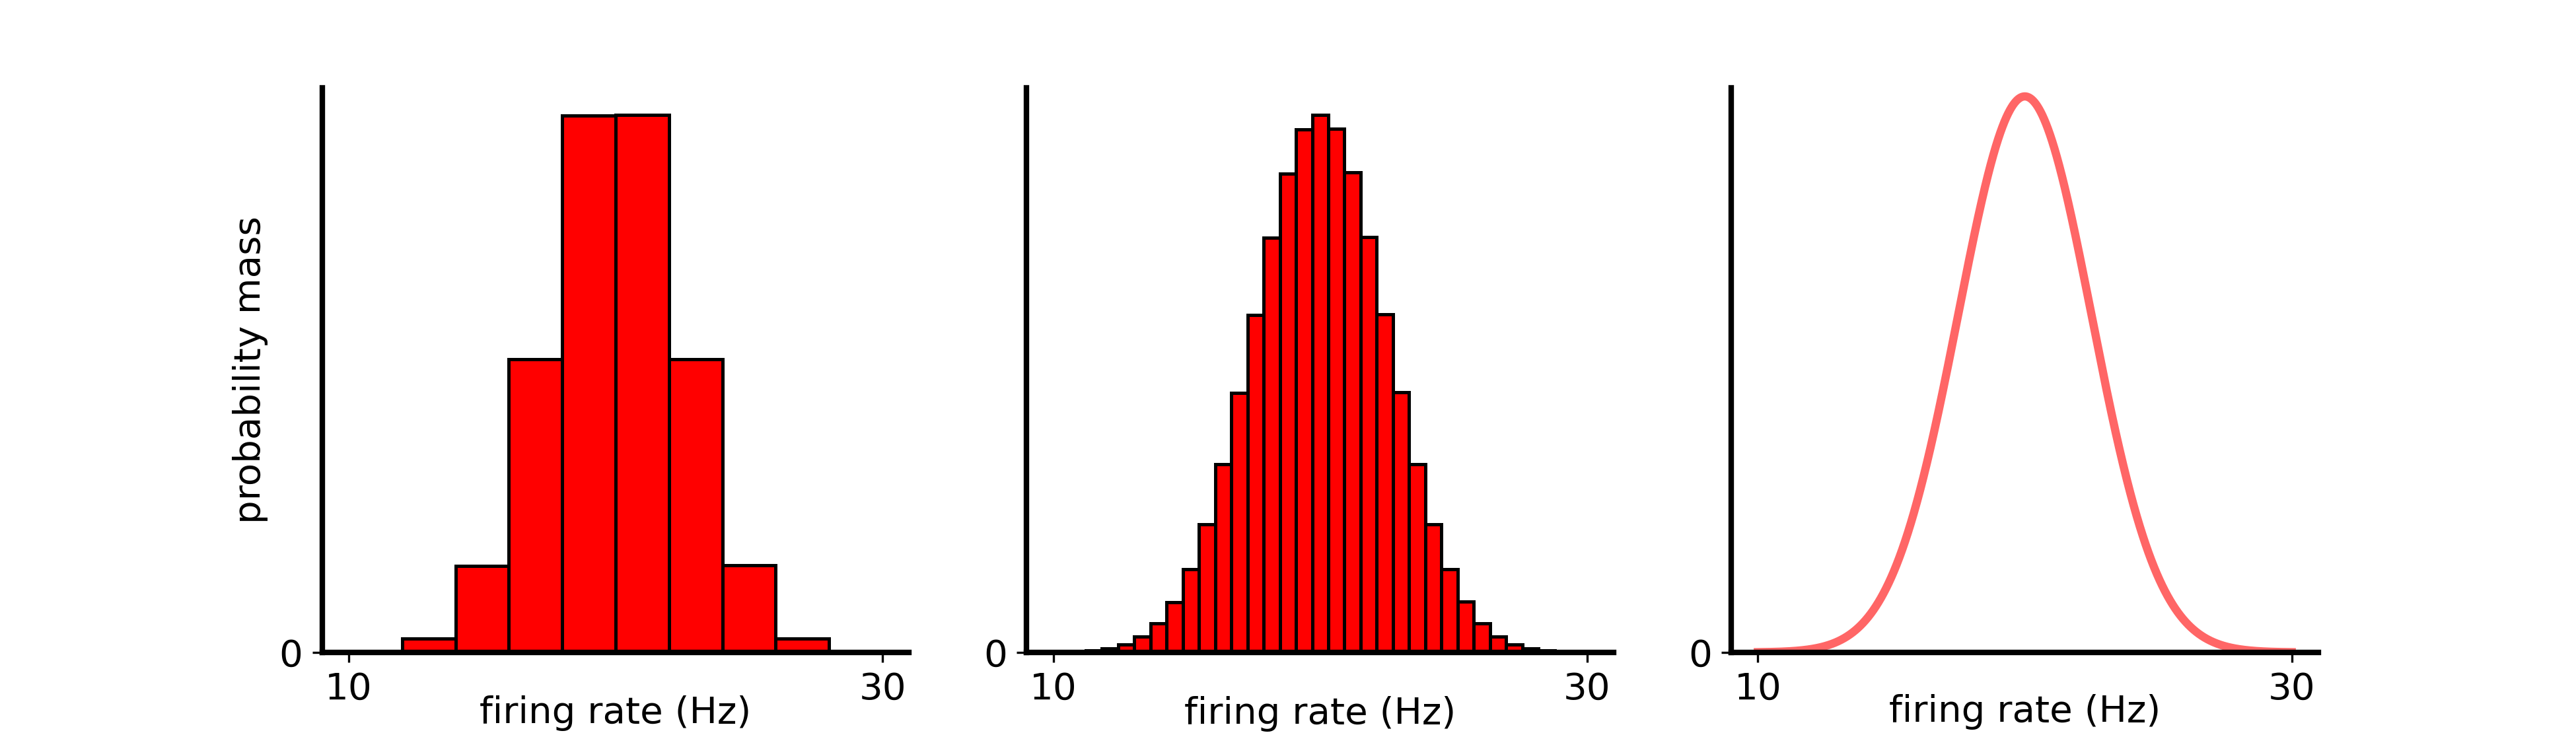
\includegraphics[height=2.5cm]{images/normal_mass_to_hist.png}
\vspace{-0.25cm}
\center 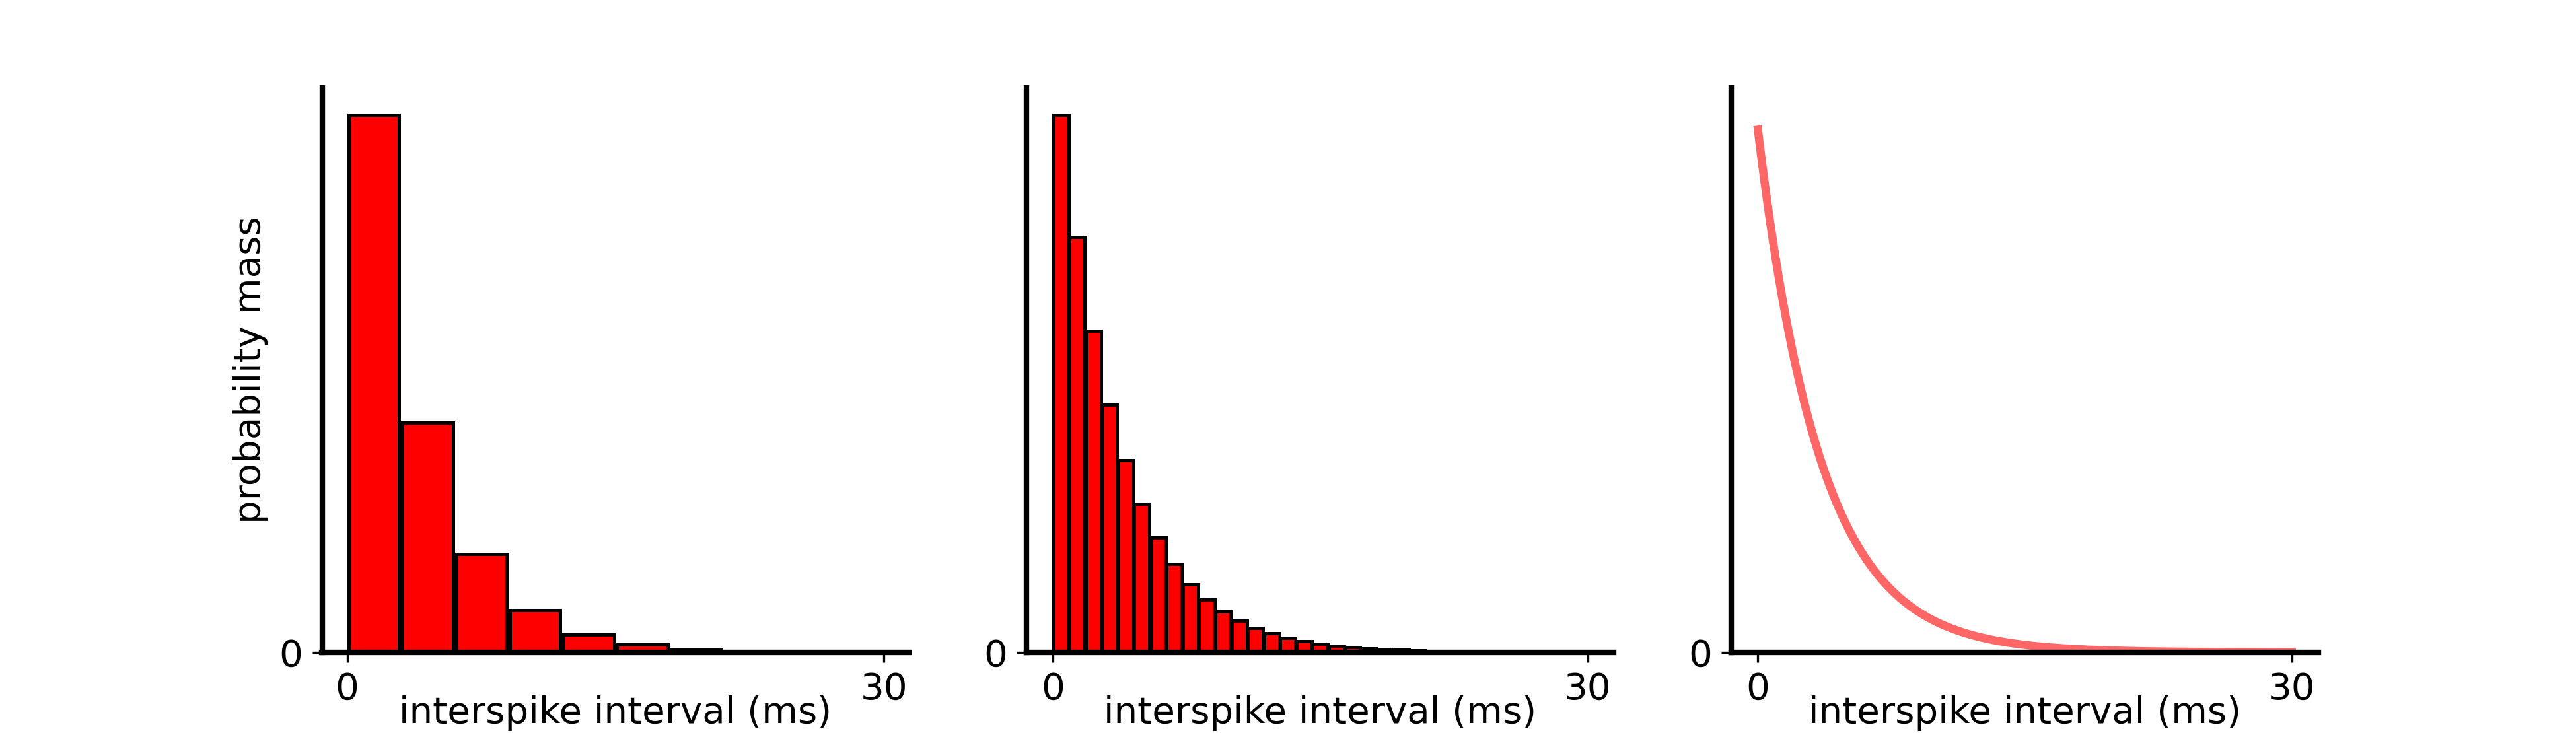
\includegraphics[height=2.5cm]{images/exp_mass_to_hist.png}

\end{frame}

%\begin{frame}
%\frametitle{Fly eye - normal stimulus distribution, CDF normal tuning curve}
%\vspace{-0.25cm}
%page 131 dayan aboot
%\end{frame}

%\begin{frame}
%\frametitle{Central Limit Theorem}
%\end{frame}

\begin{frame}
\frametitle{Probabilities as integrals}

The probability that a continuous random variable $X$ takes on a value in the interval [a, b] is given by the area under the probability density function $f(x)$.

\vspace{-0.25cm}

\begin{equation*}
P(a \leq X \leq b) = \int_a^b f(x) dx
\end{equation*}

\vspace{-0.5cm}
\begin{center}
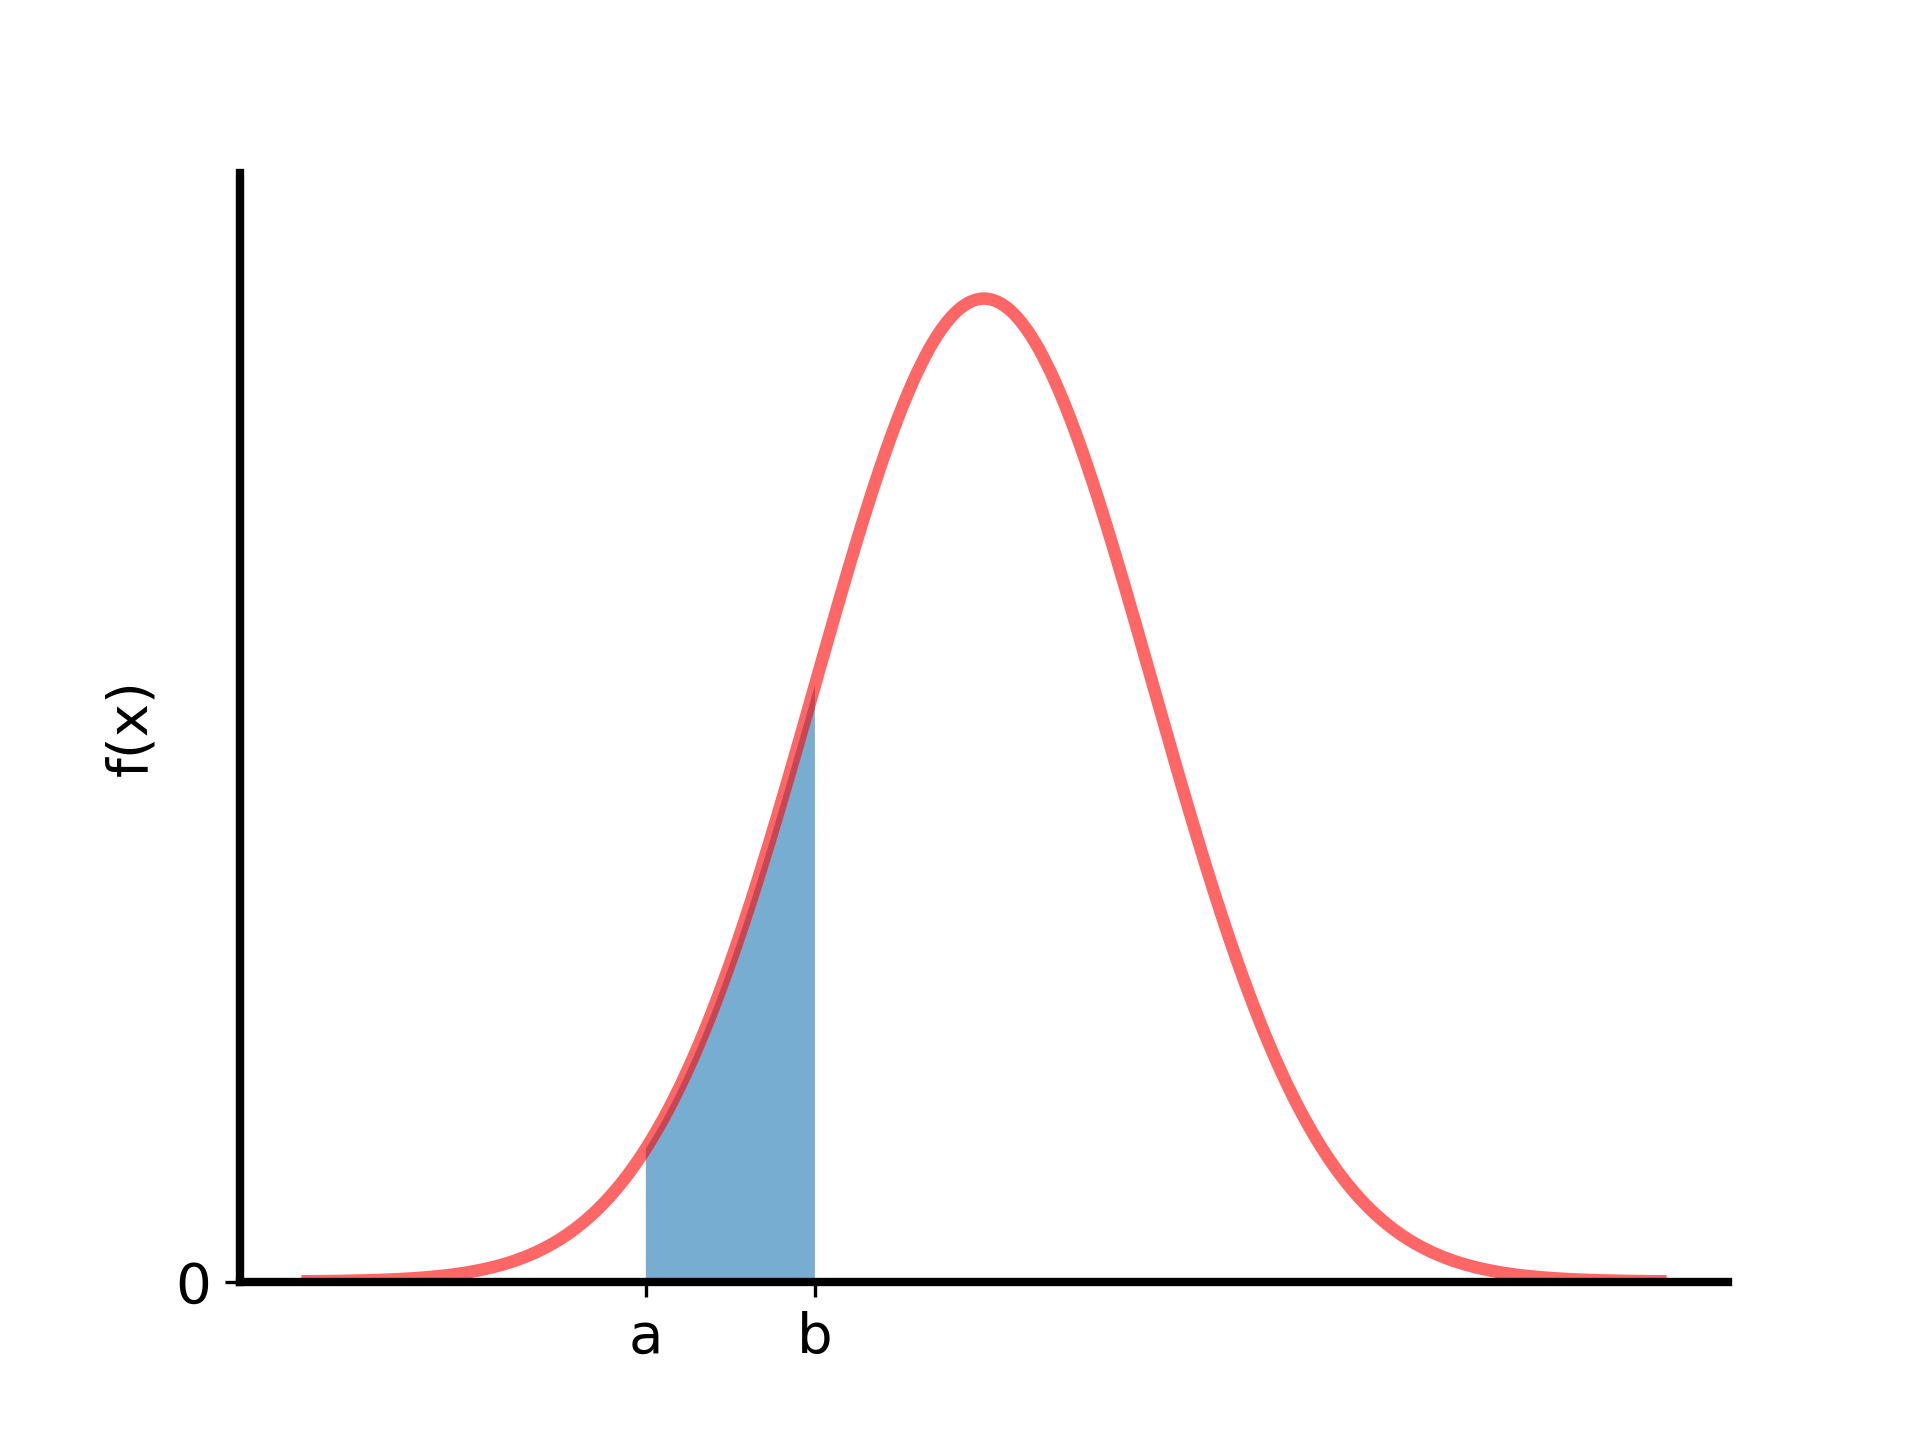
\includegraphics[height=4cm]{images/normal_area.png}
\end{center}

\end{frame}

\begin{frame}
\frametitle{The probability density function}

\begin{definition} 
A random variable $X$ is continuous if there exists a nonnegative function $f(x)$ defined on the interval $(-\infty, \infty)$, such that for any interval $[a, b]$ we have 
\begin{equation*}
P(a \leq X \leq b) = \int_a^b f(x) dx.
\end{equation*} 
\end{definition}
% \begin{theorem} This is a theorem. \end{theorem}
% \begin{proof} This is a proof. \end{proof}

\vspace{0.3cm}

\onslide<2->{
A valid probability density function (PDF) $f(x)$ has the following properties:

\begin{equation}
f(x) \geq 0 \textrm{ for all } x
\end{equation}

\begin{equation}
\int_{-\infty}^\infty f(x) dx = 1.
\end{equation}
}

\end{frame}

\begin{frame}
\frametitle{Density as probability per unit length}

The probability of a small interval $\delta$ is approximately the density
$\times \ \delta$:

\vspace{-0.3cm}

\begin{align*}
P(x \leq X \leq x + \delta) &= \int_x^{x+\delta} f(t) dt\\
& \approx f(x) \times \delta\\
\end{align*}

\vspace{-0.5cm}

\onslide<2->{
Thus density is probability per unit length (probability accumulation rate):

\begin{align*}
\frac{P(x \leq X \leq x + \delta)}{\delta} &\approx f(x) \ \ \ \ \ \ \ \ \ \ \ 
\end{align*} 
}

\end{frame}

% \begin{frame}
% \frametitle{Properties of the PDF}

% For a discrete random variable $X$, the probability mass function $p(X = x)$ satisfies:

% \begin{equation*}
% p(x) \geq 0 \textrm{ for all } x
% \end{equation*}

% \begin{equation*}
% \sum_x p(x) = 1
% \end{equation*}

% % NB these two proerties collectiveyl this implies p(x) leq to 1

% \end{frame}

\begin{frame}
\frametitle{Each possible value has zero probability}

The probability that $X$ takes on a particular value $a$ is 0, as 

\vspace{-0.25cm}

\begin{align*}
P(X = a) &= \int_a^a f(x) dx \\
&= \lim\limits_{\epsilon \to 0}  \int_{a-\epsilon}^{a+\epsilon} f(x) dx \\
&= 0.
\end{align*}

\onslide<2->{
This implies that probabilities don't depend on interval end points:

\vspace{-0.25cm}

\begin{align*}
P(a \leq X \leq b) = P(a < X < b) = P(a < X \leq b) = P(a \leq X < b),
\end{align*}

as  $P(X = a) = P(X = b) = 0$.
}

%\begin{theorem}
%$P(a \leq X \leq b) = P(a \leq X < b)$ because $P(X = b)$ = 0\\
%$P(a \leq X \leq b) = P(a < X \leq b)$ because $P(X = a)$ = 0\\
%$P(a \leq X \leq b) = P(a < X < b)$
%\end{theorem}

\end{frame}

\begin{frame}
\frametitle{Mean and variance}

The expected value (mean) of a continuous random variable $X$ is:

\begin{equation*}
\mathbb{E}[X] = \int_{-\infty}^\infty x f(x) \mathrm{d}x.
\end{equation*}

\vspace{.1cm}

\onslide<2->{
The expected value of a function $g(x)$ of $X$ is:

\begin{equation*}
\mathbb{E}[g(X)] = \int_{-\infty}^\infty g(x) f(x) \mathrm{d}x.
\end{equation*}
}

\onslide<3->{
The variance of $X$ is:

\vspace{-.4cm}

\begin{align*}
% var[X] &= \mathbb{E}[(X - \mathbb{E}[X])^2]\\
\mathrm{Var}[X] &= \mathbb{E}[(x - \mathbb{E}[X])^2] \\
&= \int_{-\infty}^\infty (x - \mathbb{E}[X])^2 f(x) \mathrm{d}x.
\end{align*}
}
% var[X] is an example of g(x)

% \begin{equation}
% var[X] = \mathbb{E}[X^2] - \mathbb{E}[X]^2
% \end{equation}

% \begin{equation}
% \mathbb{E}[X^2] = \int_{-\infty}^\infty x^2 f(x) \mathrm{d}x
% \end{equation}

% Mode

\end{frame}

\begin{frame}
\frametitle{Example: the uniform distribution}

When $X$ has a uniform distribution:

\vspace{-.3cm}

\begin{align*}
    f(x) &= 
    \begin{cases}
      \frac{1}{b-a} & \text{if}\ a \leq x \leq b \\
      0 & \text{otherwise.}
    \end{cases}
\end{align*}

\onslide<2->{
The expected value of $X$ is:

\vspace{-.3cm}

\begin{align*}
    \mathbb{E}[X] &= \int_{a}^b x \frac{1}{b-a} \mathrm{d}x = \frac{a + b}{2}.
\end{align*}
}

\onslide<3->{
The variance of $X$ is:

\vspace{-.3cm}

\begin{align*}
    \mathrm{Var}[X] &= \int_a^b \bigg(x - \frac{a + b}{2}\bigg)^2 \frac{1}{b-a} \mathrm{d}x = \frac{(b-a)^2}{12}.
\end{align*}
}

%\begin{align*}
%    \text{The PDF of a uniform distribution}\\
%    \hspace{-3cm}
%    f(x) &= 
%    \begin{cases}
%      \frac{1}{b-a} & \text{if}\ a \leq x \leq b \\
%      0 & \text{otherwise}
%    \end{cases}
%    \\[12pt]
%    \mathbb{E}[X] &= \int_{a}^b x \frac{1}{b-a} \mathrm{d}x\\
%    &= \frac{a + b}{2}
%    \\[12pt]
%    \mathrm{Var}[X] &= \int_a^b \bigg(x - \frac{a + b}{2}\bigg)^2 \frac{1}{b-a} \mathrm{d}x\\
%    &= \frac{(b-a)^2}{12}
%\end{align*}

% \begin{align*}
% \mathbb{E}[X] &= \int_{a}^b x \frac{1}{b-a} \mathrm{d}x\\
% &= \frac{a + b}{2}
% \end{align*}

% \begin{align*}
% \mathrm{Var}[X] &= \int_a^b \bigg(x - \frac{a + b}{2}\bigg)^2 \frac{1}{b-a} \mathrm{d}x\\
% &= \frac{(b-a)^2}{12}
% \end{align*}

\end{frame}


\section{Cumulative distribution functions}
\begin{frame}
\frametitle{The cumulative distribution function}

The cumulative distribution function (CDF) $F(x)$ is the area under the probability density function $f(x)$ to the left of $x$.

\center 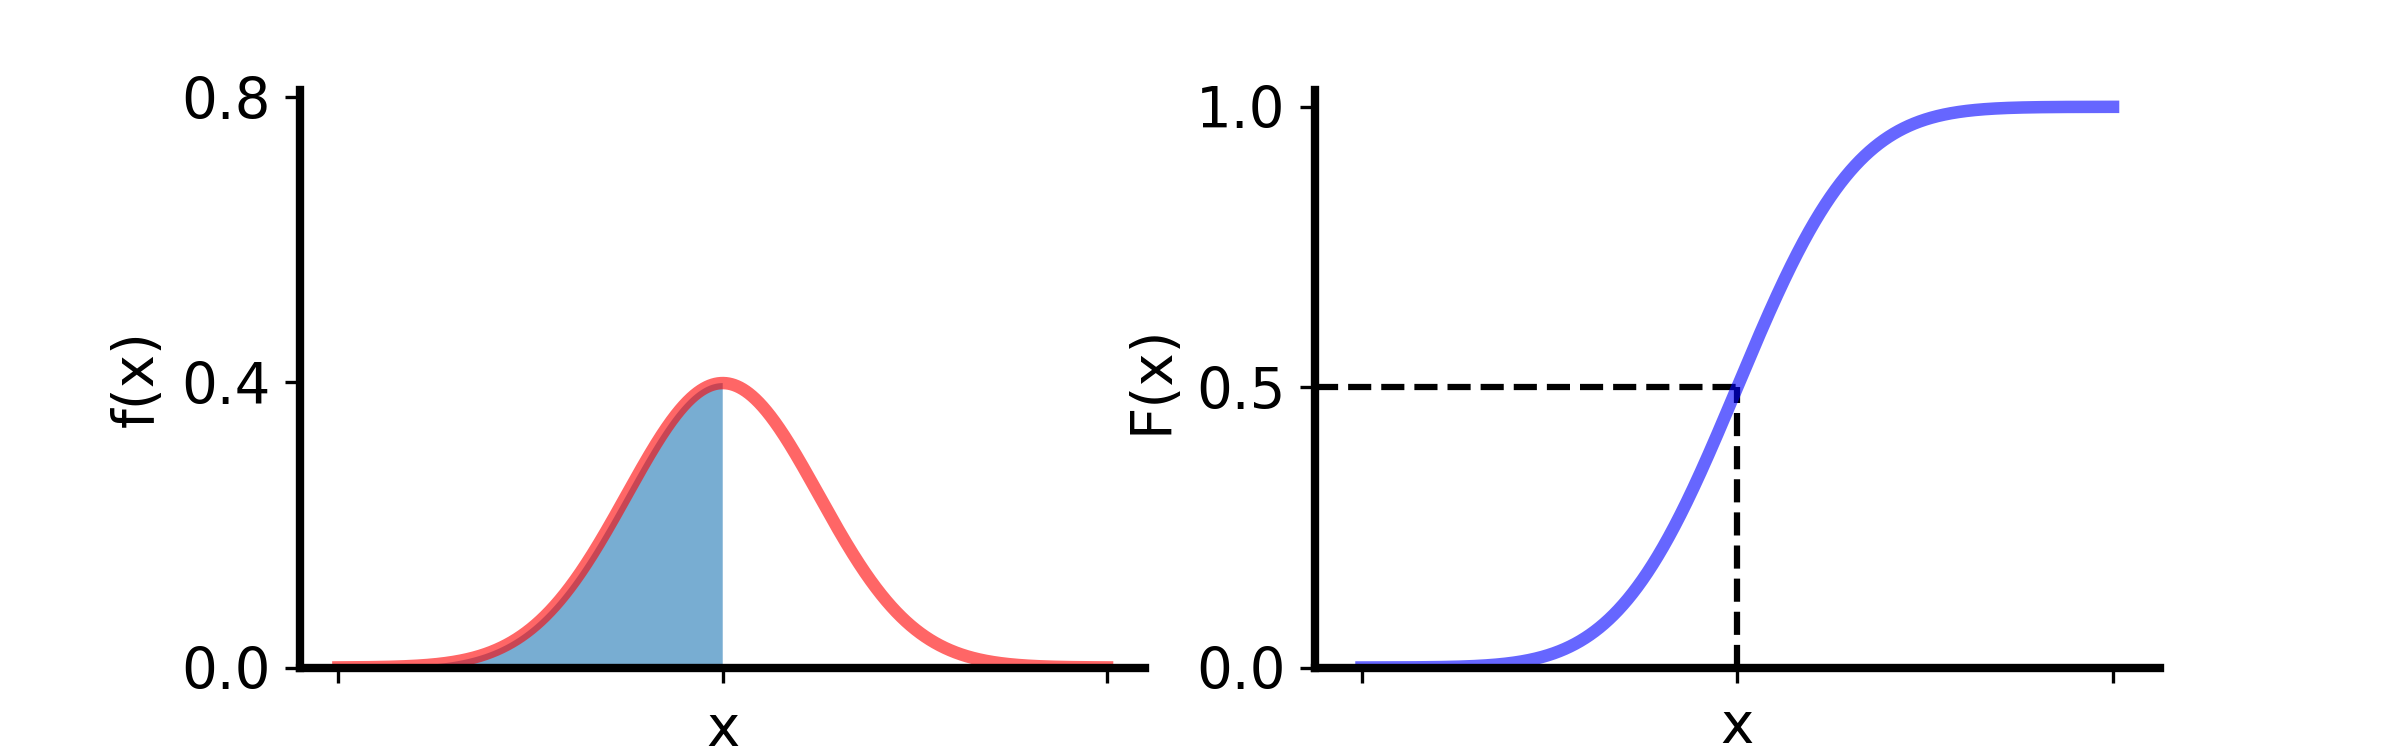
\includegraphics[height=2.5cm]{images/pdf_cdf_1.png}

\end{frame}

\begin{frame}
\frametitle{The cumulative distribution function}

%The cumulative distribution function $F(x)$ is the area under the probability density function to the left of x.

\vspace{.3cm}

\begin{definition} 
Let $X$ be a continuous random variable with probability density function $f(x)$, then the cumulative distribution function is defined as
\begin{align*}
F(x) &= P(X \leq x)\\
&= \int_{-\infty}^x f(t) dt.
\end{align*} 
\end{definition}
% \begin{theorem} This is a theorem. \end{theorem}
% \begin{proof} This is a proof. \end{proof}

\vspace{0.5cm}

\onslide<2->{
The CDF is a monotonically-increasing continuous function $F: \mathbb{R} \mapsto [0, 1]$ satisfying $\lim\limits_{x \to -\infty} F(x) = 0$ and $\lim\limits_{x \to \infty} F(x) = 1$.
}

\end{frame}

\begin{frame}
\frametitle{Computing probabilities using the CDF}

% The cumulative distribution function encodes probabilities

%For any two numbers $a$ and $b$ with $a < b$,

\vspace{-.9cm}

\begin{align*}
P(a \leq X \leq b) = F(b) - F(a).
\end{align*} 

%\vspace{-1cm}

\vspace{-.7cm}

\center 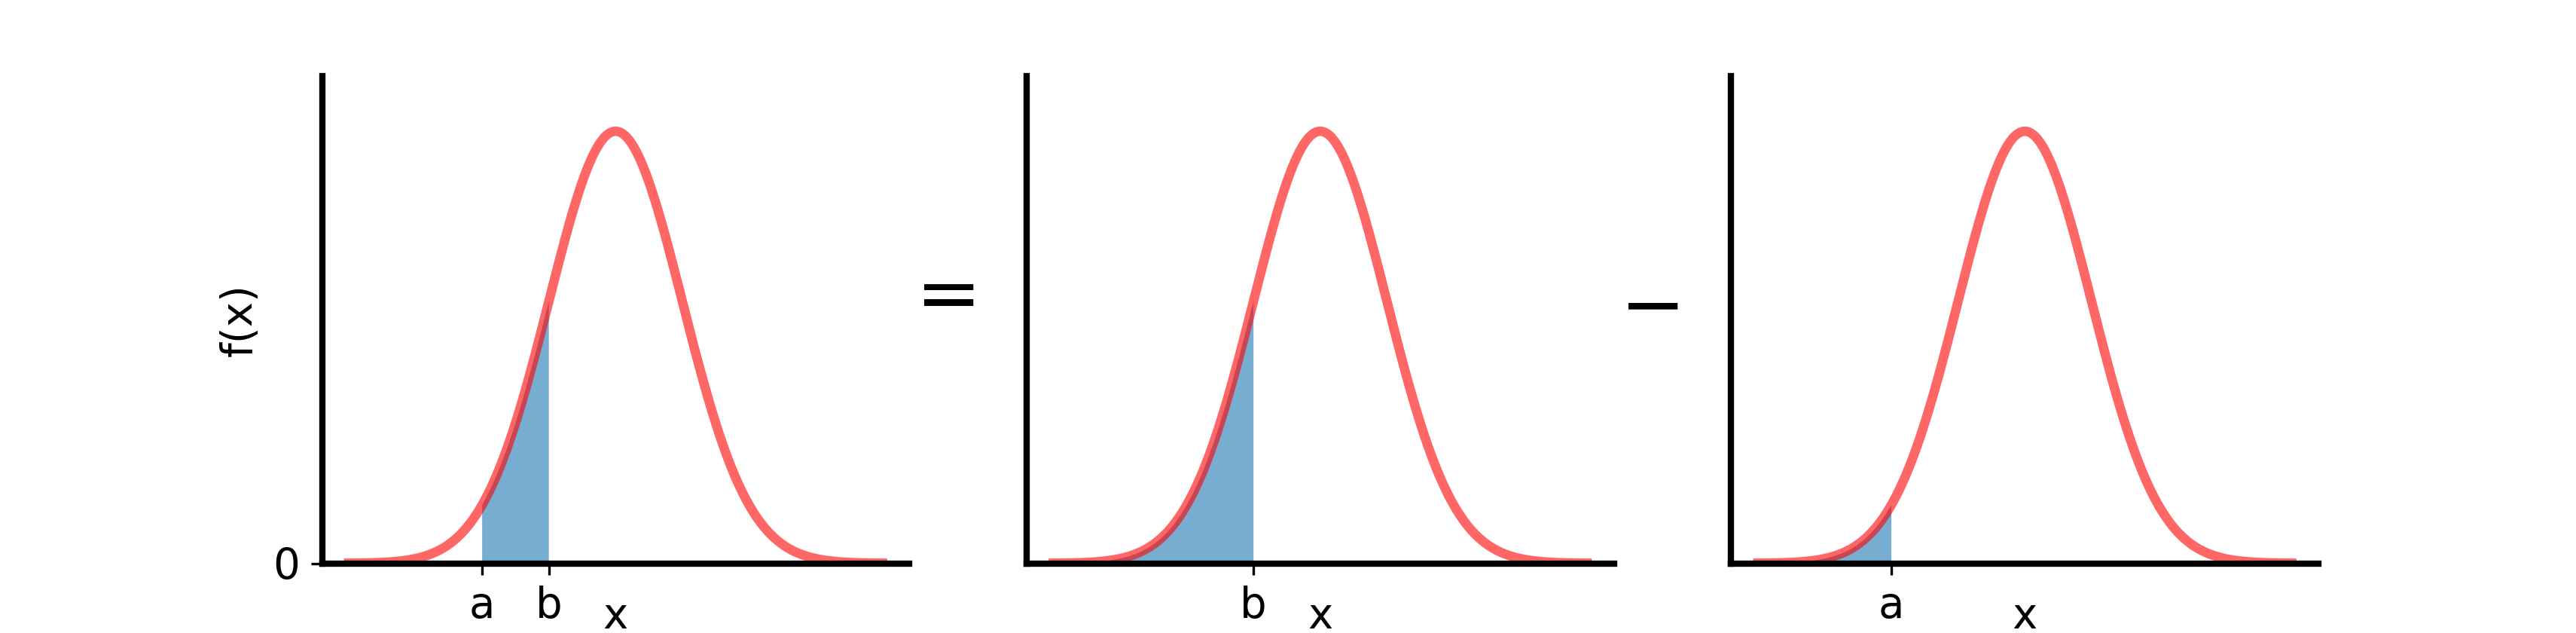
\includegraphics[height=2.5cm]{images/normal_ab_a_b.png}

\vspace{-.5cm}

%%For any number $a$,

\onslide<2->{
\begin{align*}
P(X > a) &= F(\infty) - F(a)\\
&= 1 - F(a).
\end{align*} 

\vspace{-.7cm}

\center 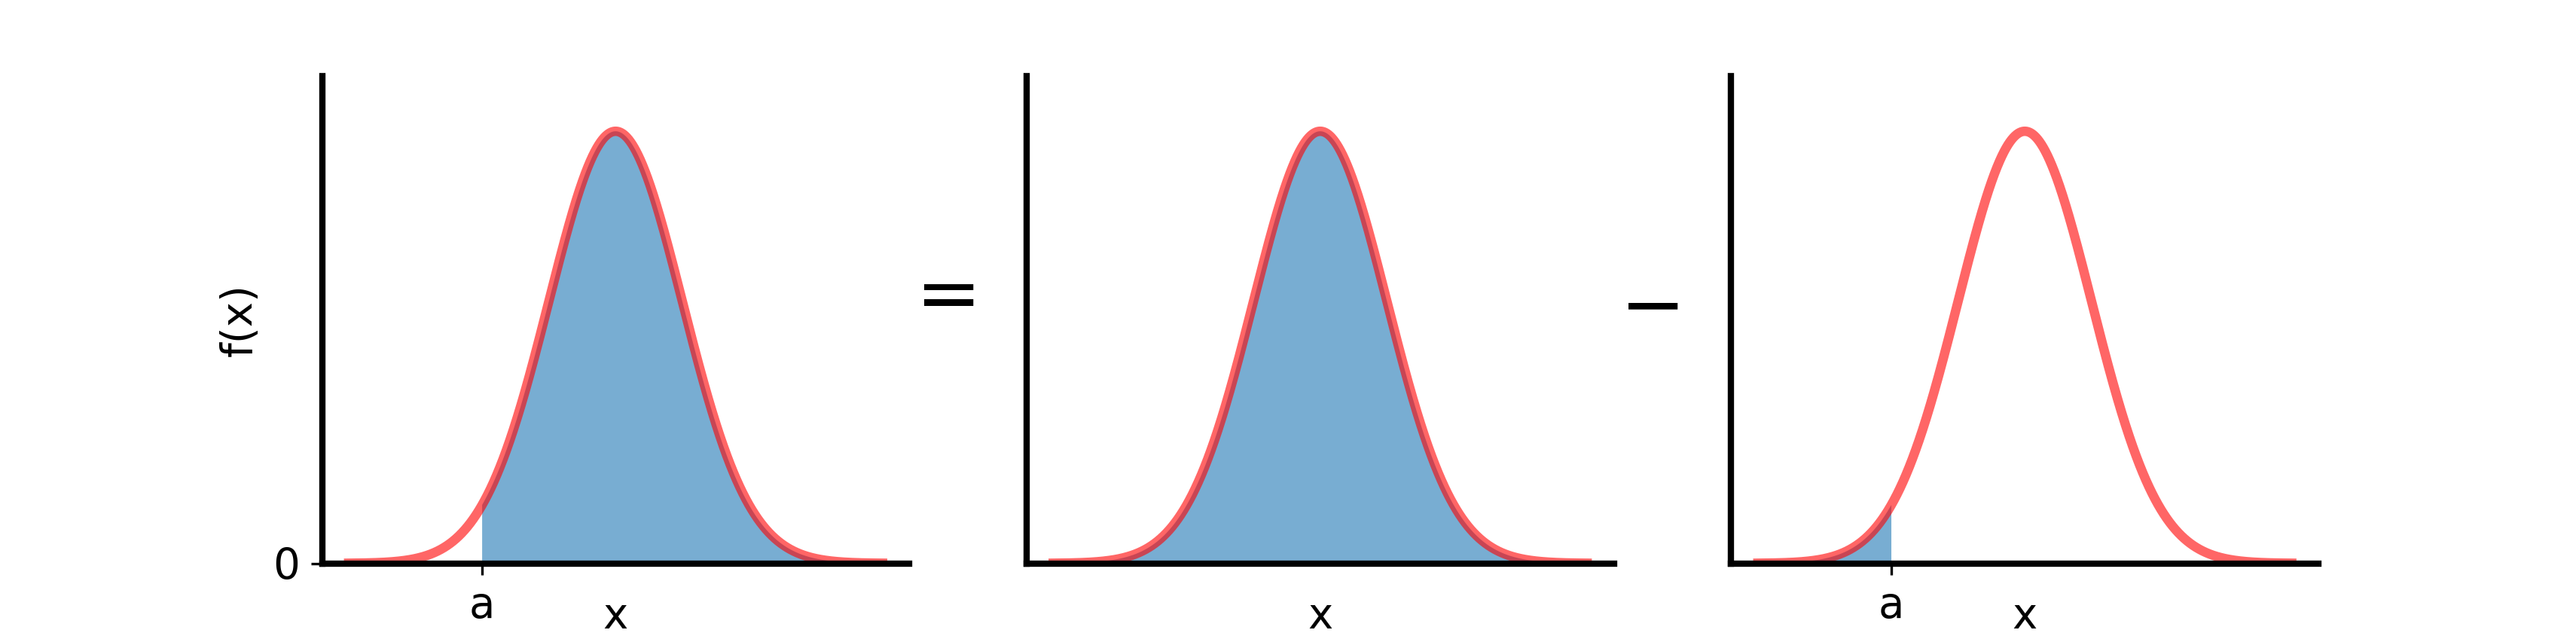
\includegraphics[height=2.5cm]{images/normal_a_inf.png}
}


%\begin{theorem}
%$P(a \leq X \leq b) = F(b) - F(a)$
%\end{theorem}
%
%\begin{proof}
%% $P(a \leq X \leq b) = P(X \leq b) - P(X < a)$\\0
%% But because $X$ is continuous, $P(X < a) = P(X \leq a)$, and so
%\begin{align*}
%P(a \leq X \leq b) &= P(X \leq b) - P(X < a)\\
%&= P(X \leq b) - P(X \leq a)\\
%&= F(b) - F(a)
%\end{align*} 
%\end{proof}

\end{frame}

\begin{frame}
\frametitle{Obtaining the PDF from the CDF}

At every $x$ at which the derivative $F^\prime(x)$ exists, $F^\prime(x) = f(x)$.

\
\onslide<2->{
\begin{examples}
When $X$ has a uniform distribution, for $a < x < b$:

\vspace{-0.3cm}

\begin{align*}
F^\prime(x) = \frac{d}{dx}\bigg(\frac{x-a}{b-a}\bigg) = \frac{1}{b-a} = f(x)
\end{align*}
\end{examples}
}
%F(x) is differentiable except at and where the graph of F(x) has sharp corners.

\end{frame}

\begin{frame}
\frametitle{Sampling using the CDF}

The inverse transform sampling algorithm can be used to sample a continuous random variable
%with arbitrary probability distribution 
using the inverse of its cumulative distribution function.

\

\onslide<2->{
Recall that $F: \mathbb{R} \mapsto [0, 1]$.
}

\ 

%To draw a sample $x$ of a continuous random variable $X$ with CDF $F$:
\onslide<3->{
To draw a sample $x \sim f(x)$:
\begin{enumerate}
    \item Sample $u \sim \U{0,1}$ (using a pseudo-random number generator)
    \item Let $x = F^{-1}(u)$
\end{enumerate}
}

\end{frame}

\begin{frame}
\frametitle{Example: the exponential distribution}

The PDF of the exponential distribution is:

\begin{equation*}
    f(x) = 
    \begin{cases}
      \lambda e ^{-\lambda x} & \text{if}\ x \geq 0 \\
      0 & \text{otherwise},
    \end{cases}
\end{equation*}

\onslide<2->{
which implies that the CDF is:

\begin{equation*}
F(x) = 1 - e^{- \lambda x} = u,
\end{equation*}
}

\onslide<3->{
and the inverse of the CDF is:

\begin{equation*}
F^{-1}(u) = -\frac{ \log(1 -u) } {\lambda}  = x.
\end{equation*}
}

\onslide<4->{
Hence, to sample $x \sim f(x)$:
\begin{enumerate}
    \item Sample $u \sim \U{0,1}$
    \item Let $x = -\frac{ \log(1 -u) } {\lambda} $
\end{enumerate}
}

\end{frame}

% If set A and set B have the same cardinality, then there is a one-to-one correspondence from set A to set B. 
% For a finite set, the cardinality of the set is the number of elements in the set.
% A set A is countably infinite if and only if set  A has the same cardinality as ℕ (the natural numbers).
% A set is countable if and only if it is finite or countably infinite.
% A set that is NOT countable is uncountable or uncountably infinite.
% A bag with infinitely many apples would be a countable infinity because (given an infinite amount of time) you can label the apples 1, 2, 3, etc.
% Uncountable is in contrast to countably infinite or countable. For example, the set of real numbers in the interval [0,1] is uncountable. There are a continuum of numbers in that interval, and that is too many to be put in a one-to-one correspondence with the natural numbers.

\section{Common distributions}
% \begin{frame}
% \frametitle{The uniform distribution}
% \end{frame}

\begin{frame}
\frametitle{The normal (Gaussian) distribution}
% An approximation to various discrete distributions.
\end{frame}

% \begin{frame}
% \frametitle{The Dirac delta}
% \end{frame}

% \begin{frame}
% \frametitle{The exponential distribution}
% \end{frame}

% \iffalse 
% CTrl + /
% %\begin{comment}
% %\section{Second section}

% \begin{frame}
% \frametitle{Highlighting text}

% In this slide, some important text will be
% \alert{highlighted} because it's important.
% Please, don't abuse it.

% \begin{block}{Remark}
% Sample text
% \end{block}

% \begin{alertblock}{Important theorem}
% Sample text in red box
% \end{alertblock}

% \begin{examples}
% Sample text in green box. The title of the block is ``Examples".
% \end{examples}
% \end{frame}
% %\end{comment}
% \fi
\end{document}